\documentclass[border=3pt,tikz]{standalone}
\usepackage{physics,bm}
\usepackage{tikz,pgfplots}
\tikzset{>=latex} % for LaTeX arrow head
\pgfplotsset{compat=1.13}
\usetikzlibrary{decorations.markings,intersections,calc}
\usepackage[outline]{contour} % glow around text
\usetikzlibrary{angles,quotes} % for pic (angle labels)
\usepackage{xcolor}
\colorlet{Ecol}{orange!90!black}
\colorlet{EcolFL}{orange!80!black}
\colorlet{Bcol}{blue!90!black}
\tikzstyle{EcolEP}=[blue!80!white]
\colorlet{veccol}{green!45!black}
\tikzstyle{charge+}=[very thin,top color=red!50,bottom color=red!90!black,shading angle=20]
\tikzstyle{charge-}=[very thin,top color=blue!50,bottom color=blue!80,shading angle=20]
\tikzstyle{vector}=[->,thick,veccol]
\tikzset{EFieldLineArrow/.style={EcolFL,decoration={markings,mark=at position #1 with {\arrow{latex}}},
                                 postaction={decorate}},
         EFieldLineArrow/.default=0.5}
\def\R{1.8}
\def\NE{8}
\def\NV{4}
\contourlength{1.6pt}



\begin{document}


% POINT CHARGE +1
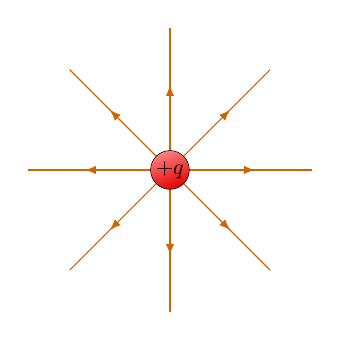
\begin{tikzpicture}
  \foreach \i [evaluate={\angle=(\i-1)*360/\NE;}] in {1,...,\NE}{
    \draw[EFieldLineArrow={0.6}] (0,0) -- (\angle:\R);
  }
  \draw[charge+] (0,0) circle (7pt) node[black,scale=0.8] {$+q$};
\end{tikzpicture}

\end{document}